\documentclass{beamer}

\usepackage[francais]{babel}
\usepackage[T1]{fontenc}
\usepackage[utf8]{inputenc}
\usepackage{beamerthemesupelec}
\usepackage{beamerouterthemesupelec}
\usepackage{beamerfontthemesupelec}
\usepackage{beamerinnerthemesupelec}
\usepackage{beamercolorthemesupelec}

\usetheme{supelec}
\useoutertheme{supelec}
\usefonttheme{supelec}
\useinnertheme{supelec}
\usecolortheme{supelec}

\title[Avancement]{Avancement du projet de visualisation}
\author{\textbf{Nicolas \textsc{Bostsarron} - Valentin \textsc{Jaouen}}}
\institute{Centrale Supélec - Campus de Rennes}

\AtBeginSection[] {
  \begin{frame}
    \frametitle{Plan}
    \tableofcontents[currentsection]
  \end{frame} 
}

\begin{document}

  \begin{frame}
    \titlepage
  \end{frame}
  
  \begin{frame}
    \frametitle{Plan}
    \tableofcontents
  \end{frame} 

  \section{Présentation du projet}
  \begin{frame}
    \frametitle{Hypothèses}
    \begin{itemize}
     \item Où : Une entreprise
     \item Quand : Réunion entre les acteurs
     \item But : Prise de décision et distribution du budget
     \item Comment : Chiffres, compte-rendus, paroles, expériences, etc...
    \end{itemize}
  \end{frame}
  
  \begin{frame}
   \frametitle{Problématiques}
   \begin{enumerate}   
    \item Les acteurs n'ont de visibilité que sur leur domaine
    \item Les acteurs ne parlent pas le même langage
    \item Une exigence peut améliorer un domaine et nuire à un autre
   \end{enumerate}
   \begin{alertblock}{Conséquence importante}
    Quelles exigences ont un réel impact positif sur l'entreprise ?
   \end{alertblock}
  \end{frame}

  \begin{frame}
    \frametitle{Réponses}
    \begin{enumerate}    
     \item Les acteurs n'ont de visibilité que sur leur domaine
     \item Les acteurs ne parlent pas le même langage
     \item Une exigence peut améliorer un domaine et nuire à un autre
    \end{enumerate}
  \end{frame}
  
  \begin{frame}
   \frametitle{Réponses}
   \begin{enumerate}
    \item Nécessité de mettre en place des indicateurs pertinents
    \item Les acteurs ne parlent pas le même langage
    \item Une exigence peut améliorer un domaine et nuire à un autre
   \end{enumerate}
  \end{frame}
  
  \begin{frame}
   \frametitle{Réponses}
   \begin{enumerate}
    \item Nécessité de mettre en place des indicateurs pertinents
    \item Nécessité de pouvoir visualiser ces indicateurs selon l'acteur
    \item Une exigence peut améliorer un domaine et nuire à un autre
   \end{enumerate}
  \end{frame}
  
  \begin{frame}
   \frametitle{Réponses}
   \begin{enumerate}
    \item Nécessité de mettre en place des indicateurs pertinents
    \item Nécessité de pouvoir visualiser ces indicateurs selon l'acteur
    \item Nécessité de lier ces indicateurs pour mesurer l'impact d'un choix
   \end{enumerate}
  \end{frame}
  
  \begin{frame}
   \frametitle{Réponses}
   \begin{enumerate}
    \item Nécessité de mettre en place des indicateurs pertinents
    \item Nécessité de pouvoir visualiser ces indicateurs selon l'acteur
    \item Nécessité de lier ces indicateurs pour mesurer l'impact d'un choix
   \end{enumerate}
   \begin{block}{Conséquence}
    Possibilité de quantifier les impacts positifs ou négatifs d'une décision sur l'ensemble des domaines
    et donc sur l'entreprise en général.
   \end{block}
  \end{frame}

  \section{Réalisations}
  \begin{frame}
   \frametitle{Choix techniques}
   \begin{itemize}
    \item Langage objet
    \item Modélisation UML
    \item Qt pour l'instant mais susceptible de changer
   \end{itemize}
  \end{frame}
  
  \begin{frame}
   \frametitle{Documentation}
   \begin{itemize}
    \item Rapports/Présentations issues de la conférence VizSec
    \item Normes ISO 27001 - 27002 - 27005
   \end{itemize}
  \end{frame}

  \begin{frame}
   \frametitle{MindMap}
   \begin{center}
    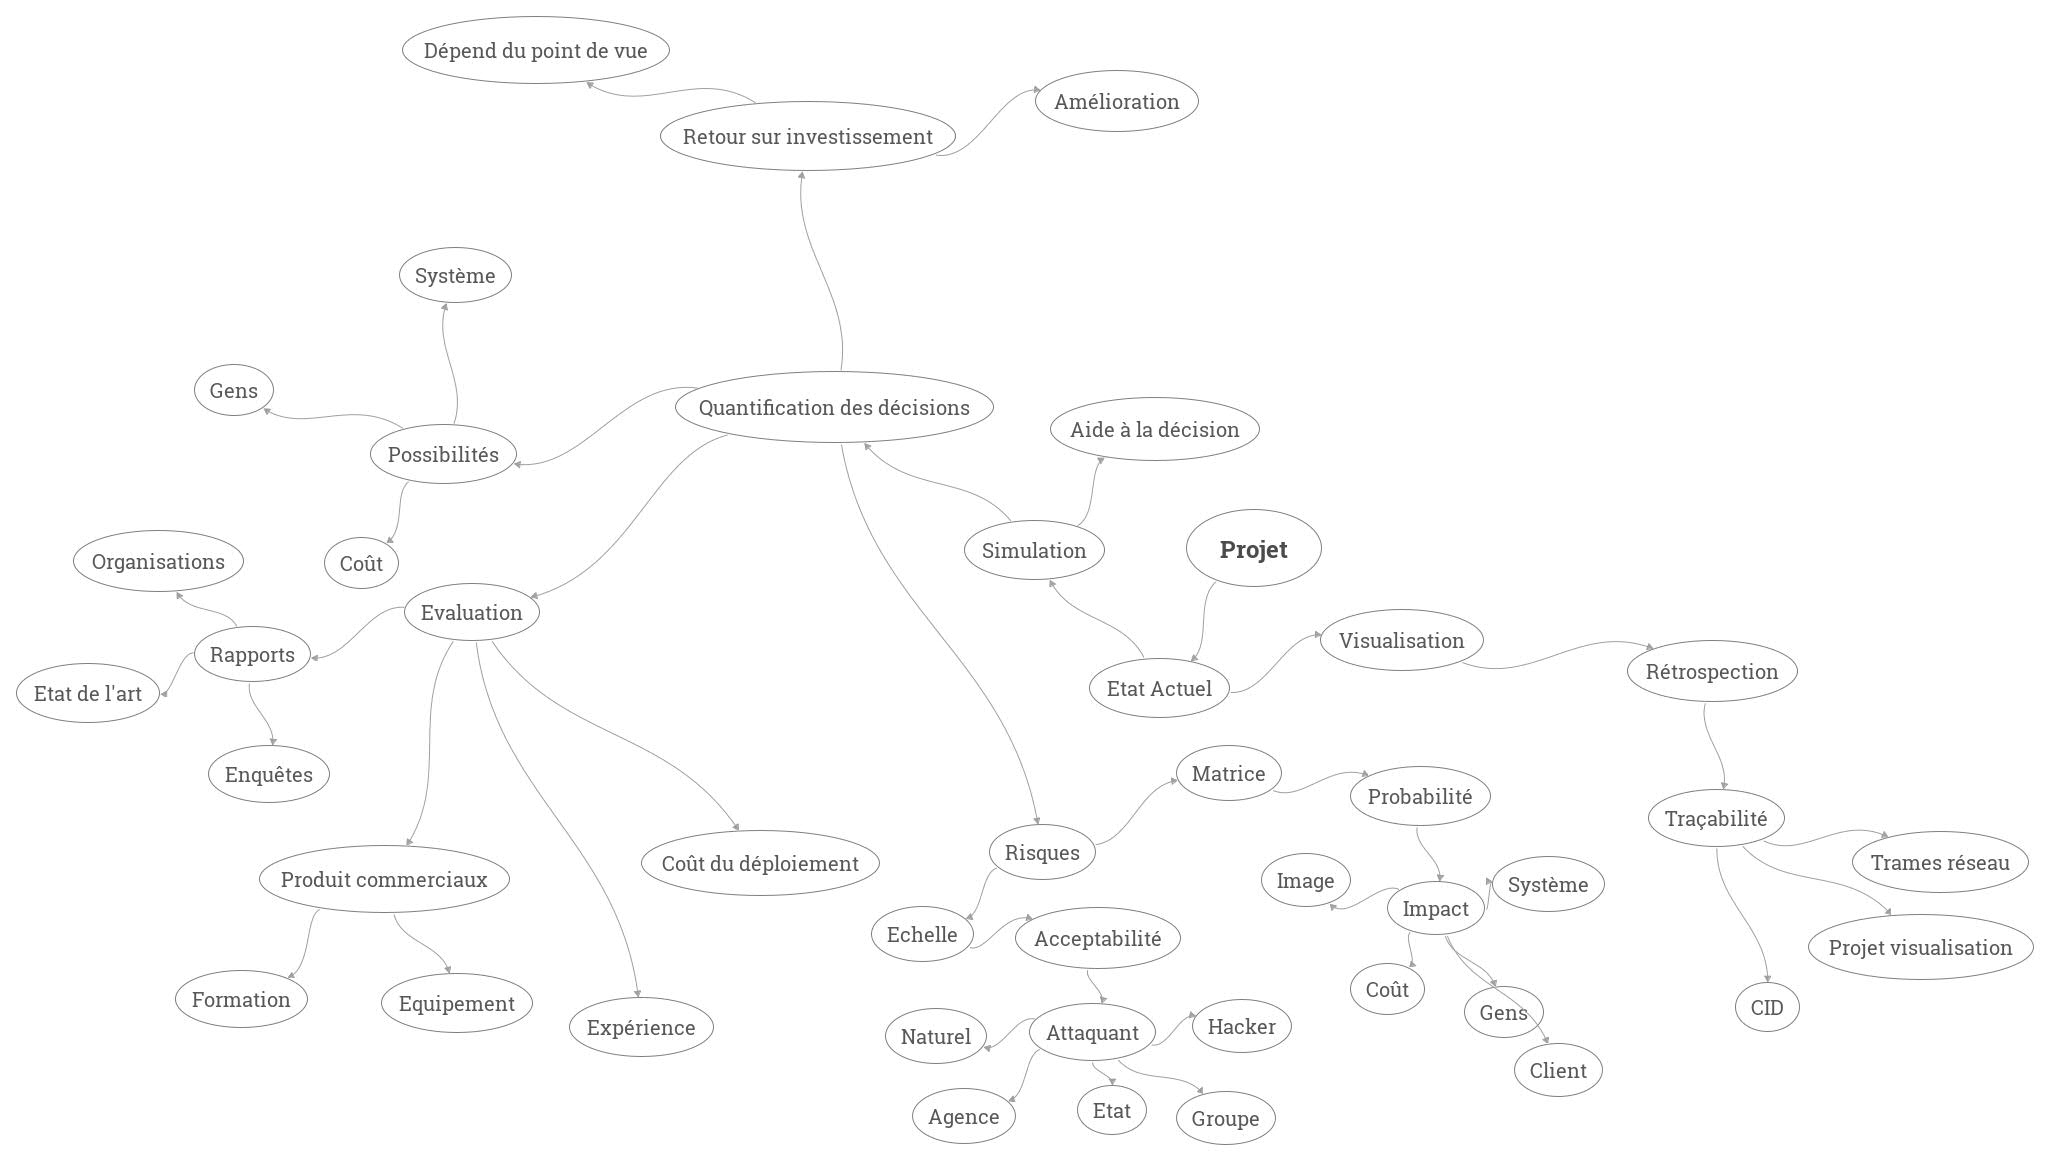
\includegraphics[scale=0.15]{mindmap.jpg}
   \end{center}
  \end{frame}
  
  \begin{frame}
   \frametitle{Modélisation UML}
   \begin{center}
    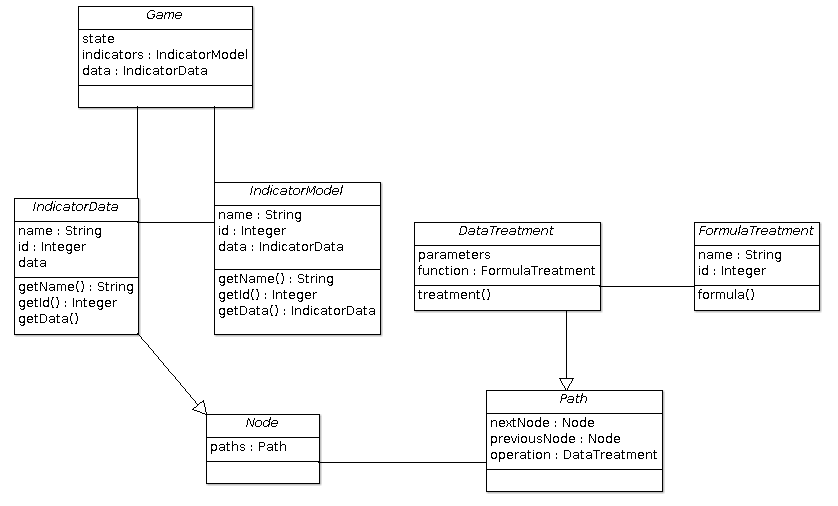
\includegraphics[scale=0.3]{uml.png}
   \end{center}

  \end{frame}
  
  \begin{frame}
   \frametitle{Questionnaire}
   \begin{itemize}
    \item Nécessité de poser les bonnes questions pour obtenir les bonnes réponses
    \item Problématique de l'évaluation
    \item Comment corréler les résultats ?
    \item Comment estimer l'impact sur les indicateurs ?
   \end{itemize}

  \end{frame}

  \section{Conclusion}
  \begin{frame}
   \frametitle{Ce qui a été fait} 
   \begin{itemize}
    \item Un mindmap
    \item Un modèle UML abstrait bien avancé
    \item Une réflexion autour d'un questionnaire à distribuer
   \end{itemize}
  \end{frame}
  
  \begin{frame}
   \frametitle{Ce qui est prévu}
   \begin{itemize}
    \item Un modèle UML abstrait complet
    \item Un modèle UML implémentable
    \item Un début d'implémentation
    \item Un questionnaire pertinent et distribué
   \end{itemize}
  \end{frame}

  \begin{frame}
    \begin{center}
      Merci de votre attention
    \end{center}
  \end{frame}

\end{document}